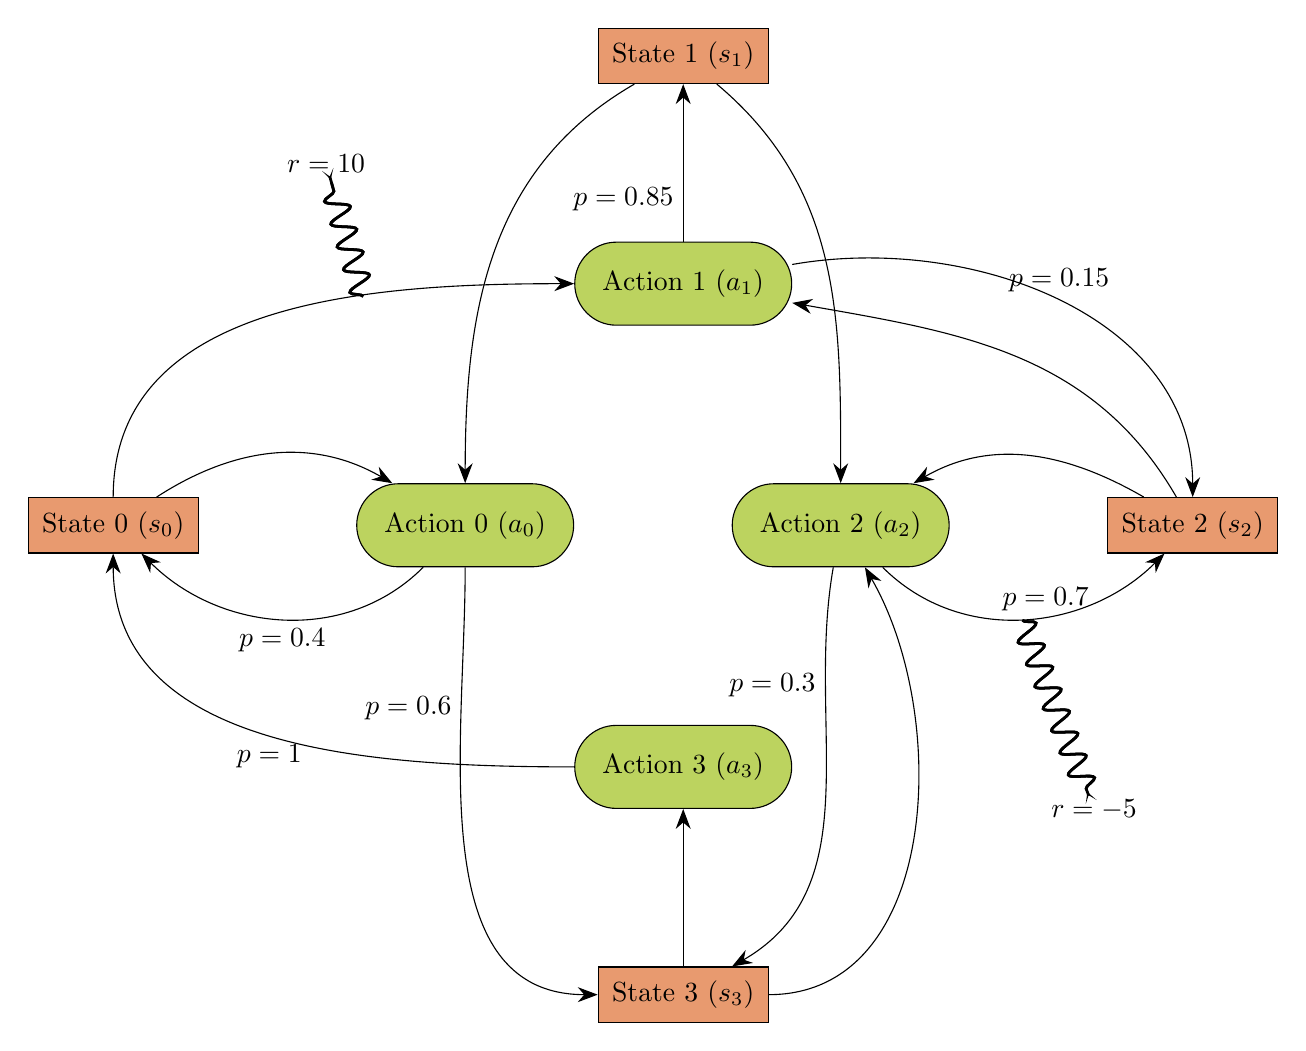
\begin{tikzpicture}
	\usetikzlibrary{arrows, automata, positioning, arrows.meta, decorations.pathreplacing, decorations.markings}
	
	\definecolor{statecolor}{HTML}{e89a6f};
	\definecolor{actioncolor}{HTML}{bcd35f};
	\tikzset{
		state/.style={
			shape=rectangle,
			draw=black,
			fill=statecolor,
			align=center,
			minimum height=2em,
			minimum width=4em,
			inner sep=5pt,
		},
		action/.style={
			shape=rectangle,
			draw=black,
			fill=actioncolor,
			align=center,
			inner sep=10pt,
			rounded corners=15pt,
		},
		reward/.style={
			decorate,
			decoration={snake, amplitude=1.5mm, segment length=3mm},
			line width=1pt,
			postaction={draw, -{Stealth[scale=-0.5]}}
		},
		transition/.style={
			->,
			>={Stealth[scale=1.5]},
		}
	};
	\tikzset{node distance=2cm and 2cm}
	\node[state] (s0) {State 0 ($s_0$)};
	\node[action, right=2cm of s0] (a0) {Action 0 ($a_0$)};
	\node[action, above right=2cm and 0cm of a0] (a1) {Action 1 ($a_1$)};
	\node[action, right=2cm of a0] (a2) {Action 2 ($a_2$)};
	\node[action, below right=2cm and 0cm of a0] (a3) {Action 3 ($a_3$)};
	\node[state, above=2cm of a1] (s1) {State 1 ($s_1$)};
	\node[state, right=2cm of a2] (s2) {State 2 ($s_2$)};
	\node[state, below=2cm of a3] (s3) {State 3 ($s_3$)};
	
	\node[draw=none, above right=2.3cm and 2cm of s0] (r0s) {};
	\node[draw=none, above right=4cm and 1cm of s0] (r0e) {$r=10$};
	
	\node[draw=none, below left=0.6cm and 1cm of s2] (r1s) {};
	\node[draw=none, below left=3cm and -0.5cm of s2] (r1e) {$r=-5$};
	
	\begin{scope} % actions
		\draw[transition] 
		(s0) 
		to[in=150, out=33]
		(a0);
		
		\draw[transition] 
		(s0) 
		to[in=180, out=90]
		(a1);
		
		\draw[transition] 
		(s1) 
		to[in=90, out=320]
		(a2);
		
		\draw[transition] 
		(s1) 
		to[in=90, out=210]
		(a0);
		
		\draw[transition] 
		(s2) 
		to[in=350, out=120]
		(a1);
		
		\draw[transition] 
		(s2) 
		to[in=30, out=150]
		(a2);
		
		\draw[transition] 
		(s3) 
		to
		(a3);
		
		\draw[transition] 
		(s3) 
		to[in=300, out=00]
		(a2);		
	\end{scope}
	
	\begin{scope} % transitions
		\draw[transition] 
		(a0)
		to[in=315, out=225] node[midway, below] 
		{$p = 0.4$} 
		(s0);
		
		\draw[transition] 
		(a0)
		to[in=180, out=270] node[near start, left] 
		{$p = 0.6$} 
		(s3);
		
		\draw[transition] 
		(a1) 
		to[in=270, out=90] node[near start, left] 
		{$p = 0.85$} 
		(s1);
		
		\draw[transition] 
		(a1) 
		to[in=90, out=10] node[midway, above]
		{$p = 0.15$} 
		(s2);
		
		\draw[transition] 
		(a2) 
		to[in=225, out=315] node[near end, left] 
		{$p = 0.7$} 
		(s2);
		
		\draw[transition] 
		(a2) 
		to[in=30, out=260] node[near start, left] 
		{$p = 0.3$} 
		(s3);
		
		\draw[transition] 
		(a3) 
		to[in=270, out=180] node[midway, below] 
		{$p = 1$} 
		(s0);
		
	\end{scope}
	
	\begin{scope}
		\draw[reward]
		(r0s)
		to
		(r0e);
		
		\draw[reward]
		(r1s)
		to
		(r1e);
		
	\end{scope}
\end{tikzpicture}